% Options for packages loaded elsewhere
\PassOptionsToPackage{unicode}{hyperref}
\PassOptionsToPackage{hyphens}{url}
\documentclass[
  11pt,
]{article}
\usepackage{xcolor}
\usepackage[margin=2.5cm]{geometry}
\usepackage{amsmath,amssymb}
\setcounter{secnumdepth}{5}
\usepackage{iftex}
\ifPDFTeX
  \usepackage[T1]{fontenc}
  \usepackage[utf8]{inputenc}
  \usepackage{textcomp} % provide euro and other symbols
\else % if luatex or xetex
  \usepackage{unicode-math} % this also loads fontspec
  \defaultfontfeatures{Scale=MatchLowercase}
  \defaultfontfeatures[\rmfamily]{Ligatures=TeX,Scale=1}
\fi
\usepackage{lmodern}
\ifPDFTeX\else
  % xetex/luatex font selection
  \setmainfont[]{Arial}
\fi
% Use upquote if available, for straight quotes in verbatim environments
\IfFileExists{upquote.sty}{\usepackage{upquote}}{}
\IfFileExists{microtype.sty}{% use microtype if available
  \usepackage[]{microtype}
  \UseMicrotypeSet[protrusion]{basicmath} % disable protrusion for tt fonts
}{}
\makeatletter
\@ifundefined{KOMAClassName}{% if non-KOMA class
  \IfFileExists{parskip.sty}{%
    \usepackage{parskip}
  }{% else
    \setlength{\parindent}{0pt}
    \setlength{\parskip}{6pt plus 2pt minus 1pt}}
}{% if KOMA class
  \KOMAoptions{parskip=half}}
\makeatother
\usepackage{color}
\usepackage{fancyvrb}
\newcommand{\VerbBar}{|}
\newcommand{\VERB}{\Verb[commandchars=\\\{\}]}
\DefineVerbatimEnvironment{Highlighting}{Verbatim}{commandchars=\\\{\}}
% Add ',fontsize=\small' for more characters per line
\usepackage{framed}
\definecolor{shadecolor}{RGB}{248,248,248}
\newenvironment{Shaded}{\begin{snugshade}}{\end{snugshade}}
\newcommand{\AlertTok}[1]{\textcolor[rgb]{0.94,0.16,0.16}{#1}}
\newcommand{\AnnotationTok}[1]{\textcolor[rgb]{0.56,0.35,0.01}{\textbf{\textit{#1}}}}
\newcommand{\AttributeTok}[1]{\textcolor[rgb]{0.13,0.29,0.53}{#1}}
\newcommand{\BaseNTok}[1]{\textcolor[rgb]{0.00,0.00,0.81}{#1}}
\newcommand{\BuiltInTok}[1]{#1}
\newcommand{\CharTok}[1]{\textcolor[rgb]{0.31,0.60,0.02}{#1}}
\newcommand{\CommentTok}[1]{\textcolor[rgb]{0.56,0.35,0.01}{\textit{#1}}}
\newcommand{\CommentVarTok}[1]{\textcolor[rgb]{0.56,0.35,0.01}{\textbf{\textit{#1}}}}
\newcommand{\ConstantTok}[1]{\textcolor[rgb]{0.56,0.35,0.01}{#1}}
\newcommand{\ControlFlowTok}[1]{\textcolor[rgb]{0.13,0.29,0.53}{\textbf{#1}}}
\newcommand{\DataTypeTok}[1]{\textcolor[rgb]{0.13,0.29,0.53}{#1}}
\newcommand{\DecValTok}[1]{\textcolor[rgb]{0.00,0.00,0.81}{#1}}
\newcommand{\DocumentationTok}[1]{\textcolor[rgb]{0.56,0.35,0.01}{\textbf{\textit{#1}}}}
\newcommand{\ErrorTok}[1]{\textcolor[rgb]{0.64,0.00,0.00}{\textbf{#1}}}
\newcommand{\ExtensionTok}[1]{#1}
\newcommand{\FloatTok}[1]{\textcolor[rgb]{0.00,0.00,0.81}{#1}}
\newcommand{\FunctionTok}[1]{\textcolor[rgb]{0.13,0.29,0.53}{\textbf{#1}}}
\newcommand{\ImportTok}[1]{#1}
\newcommand{\InformationTok}[1]{\textcolor[rgb]{0.56,0.35,0.01}{\textbf{\textit{#1}}}}
\newcommand{\KeywordTok}[1]{\textcolor[rgb]{0.13,0.29,0.53}{\textbf{#1}}}
\newcommand{\NormalTok}[1]{#1}
\newcommand{\OperatorTok}[1]{\textcolor[rgb]{0.81,0.36,0.00}{\textbf{#1}}}
\newcommand{\OtherTok}[1]{\textcolor[rgb]{0.56,0.35,0.01}{#1}}
\newcommand{\PreprocessorTok}[1]{\textcolor[rgb]{0.56,0.35,0.01}{\textit{#1}}}
\newcommand{\RegionMarkerTok}[1]{#1}
\newcommand{\SpecialCharTok}[1]{\textcolor[rgb]{0.81,0.36,0.00}{\textbf{#1}}}
\newcommand{\SpecialStringTok}[1]{\textcolor[rgb]{0.31,0.60,0.02}{#1}}
\newcommand{\StringTok}[1]{\textcolor[rgb]{0.31,0.60,0.02}{#1}}
\newcommand{\VariableTok}[1]{\textcolor[rgb]{0.00,0.00,0.00}{#1}}
\newcommand{\VerbatimStringTok}[1]{\textcolor[rgb]{0.31,0.60,0.02}{#1}}
\newcommand{\WarningTok}[1]{\textcolor[rgb]{0.56,0.35,0.01}{\textbf{\textit{#1}}}}
\usepackage{longtable,booktabs,array}
\newcounter{none} % for unnumbered tables
\usepackage{calc} % for calculating minipage widths
% Correct order of tables after \paragraph or \subparagraph
\usepackage{etoolbox}
\makeatletter
\patchcmd\longtable{\par}{\if@noskipsec\mbox{}\fi\par}{}{}
\makeatother
% Allow footnotes in longtable head/foot
\IfFileExists{footnotehyper.sty}{\usepackage{footnotehyper}}{\usepackage{footnote}}
\makesavenoteenv{longtable}
\usepackage{graphicx}
\makeatletter
\newsavebox\pandoc@box
\newcommand*\pandocbounded[1]{% scales image to fit in text height/width
  \sbox\pandoc@box{#1}%
  \Gscale@div\@tempa{\textheight}{\dimexpr\ht\pandoc@box+\dp\pandoc@box\relax}%
  \Gscale@div\@tempb{\linewidth}{\wd\pandoc@box}%
  \ifdim\@tempb\p@<\@tempa\p@\let\@tempa\@tempb\fi% select the smaller of both
  \ifdim\@tempa\p@<\p@\scalebox{\@tempa}{\usebox\pandoc@box}%
  \else\usebox{\pandoc@box}%
  \fi%
}
% Set default figure placement to htbp
\def\fps@figure{htbp}
\makeatother
\setlength{\emergencystretch}{3em} % prevent overfull lines
\providecommand{\tightlist}{%
  \setlength{\itemsep}{0pt}\setlength{\parskip}{0pt}}
\usepackage{fancyhdr}
\pagestyle{fancy}
% Ne pas inclure de logos dans l'en-tête par défaut
\fancyhead{}
% Vous pouvez conserver le pied de page avec le numéro de page si vous le souhaitez
\fancyfoot[C]{\thepage}
% Assurez-vous que la hauteur de l'en-tête est correcte
\setlength{\headheight}{15pt}
\usepackage{booktabs}
\usepackage{longtable}
\usepackage{array}
\usepackage{multirow}
\usepackage{wrapfig}
\usepackage{float}
\usepackage{colortbl}
\usepackage{pdflscape}
\usepackage{tabu}
\usepackage{threeparttable}
\usepackage{threeparttablex}
\usepackage[normalem]{ulem}
\usepackage{makecell}
\usepackage{xcolor}
\usepackage{bookmark}
\IfFileExists{xurl.sty}{\usepackage{xurl}}{} % add URL line breaks if available
\urlstyle{same}
\hypersetup{
  hidelinks,
  pdfcreator={LaTeX via pandoc}}

\author{}
\date{\vspace{-2.5em}}

\begin{document}

\begin{titlepage}
\begin{center}

\begin{minipage}{0.15\textwidth}

\includegraphics[width=\linewidth]{logo_ansd}
\end{minipage}
\hfill
\begin{minipage}{0.15\textwidth}

\includegraphics[width=\linewidth]{logo_ensae}
\end{minipage}

\vspace{2cm}

{\Huge\bfseries TP1 : Profil démographique des ménages nigérians \par}
\vspace{1.5cm}

{\Large\textbf{Rapport d'analyse}}\par
\vspace{1.5cm}

\textbf{Auteurs :}\par
\vspace{0.5cm}
Mouhamet SECK\\
\vspace{0.2cm}
Manampisoa Clarrat FINARITRINIAINA\\

\vfill

{\Large Projet statistique avec R ou python}\\
\vspace{1cm}
{\large ENSAE - ISE1-CL / ISE1 MATH - Mars 2026}

\vspace{1cm}

\end{center}
\end{titlepage}

{
\setcounter{tocdepth}{2}
\tableofcontents
}
\newpage

\section{Introduction}\label{introduction}

Ce rapport présente les analyses descriptives et les tests statistiques
réalisés dans le cadre du TP1, à partir des données de la Nigeria
General Household Survey (GHS) Panel -- vague 4 (2018--2019). L'objectif
est d'étudier le profil démographique des ménages nigérians : structure
par âge, répartition par sexe, liens de parenté, taille des ménages et
disparités entre milieux rural et urbain.

\section{Méthodologie}\label{muxe9thodologie}

\subsection{Données et Variables
Clés}\label{donnuxe9es-et-variables-cluxe9s}

Les fichiers suivants ont été utilisés :

\begin{itemize}
\item
  \textbf{sect1\_harvestw4.dta} : 30 337 individus, variables
  démographiques (sexe, âge, lien de parenté, secteur).
\item
  \textbf{secta\_harvestw4.dta} : 5 025 ménages, informations de
  couverture (utilisé pour vérifier la cohérence des identifiants).
\end{itemize}

Les variables clés retenues sont :

\begin{itemize}
\item
  \textbf{Sexe} : \texttt{s1q2} (1 = MALE, 2 = FEMALE).
\item
  \textbf{Âge} : \texttt{s1q4} (en années).
\item
  \textbf{Lien de parenté} : \texttt{s1q3} (recodé en quatre catégories
  : Chef, Conjoint, Enfant, Autre).
\item
  \textbf{Milieu de résidence} : \texttt{sector} (1 = Urban, 2 = Rural).
\item
  \textbf{Taille du ménage} : calculée comme le nombre d'individus par
  \texttt{hhid}.
\end{itemize}

\subsection{Traitements Effectués}\label{traitements-effectuuxe9s}

\begin{Shaded}
\begin{Highlighting}[]
\CommentTok{\# Exploration : vérification des doublons, analyse des valeurs manquantes,}
\CommentTok{\# cohérence des identifiants}

\CommentTok{\# Analyse univariée de l\textquotesingle{}âge : statistiques descriptives,}
\CommentTok{\# test de normalité de Shapiro{-}Wilk, histogramme, boxplot}

\CommentTok{\# Pyramide des âges : groupes quinquennaux, effectifs par sexe}

\CommentTok{\# Lien de parenté : fréquences, intervalles de confiance à 95 \%, barplot}

\CommentTok{\# Taille des ménages : comparaison rural/urbain (statistiques,}
\CommentTok{\# test de Wilcoxon, taille d\textquotesingle{}effet, boxplot, violin plot)}

\CommentTok{\# Tableau récapitulatif : âge, sexe, taille du ménage stratifiés par zone,}
\CommentTok{\# avec tests de comparaison}
\end{Highlighting}
\end{Shaded}

Les traitements réalisés comprennent l'exploration des fichiers
(vérification des doublons, analyse des valeurs manquantes, cohérence
des identifiants), l'analyse univariée de l'âge avec test de normalité
de Shapiro-Wilk, la construction de la pyramide des âges par groupes
quinquennaux, l'analyse des liens de parenté avec intervalles de
confiance à 95 \%, la comparaison de la taille des ménages entre milieux
rural et urbain via un test de Wilcoxon-Mann-Whitney, et un tableau
récapitulatif stratifié par zone de résidence.

\section{Résultats}\label{ruxe9sultats}

\subsection{Qualité des Données et Valeurs
Manquantes}\label{qualituxe9-des-donnuxe9es-et-valeurs-manquantes}

L'examen des valeurs manquantes sur les variables clés révèle une
situation très satisfaisante. Dans \texttt{sect1\_w4}, les variables
démographiques \texttt{s1q2} (sexe), \texttt{s1q4} (âge) et
\texttt{s1q3} (lien de parenté) présentent moins de 1 \% de valeurs
manquantes, principalement pour les individus partis ou non membres du
ménage, ce qui est structurellement attendu. La variable \texttt{sector}
(milieu de résidence) est complète. Par ailleurs, 4 980 ménages sont
communs entre \texttt{sect1} et \texttt{secta} sur les 5 025 de
\texttt{secta}, confirmant la cohérence des identifiants. Aucun doublon
n'a été détecté sur la clé (\texttt{hhid}, \texttt{indiv}). Les quelques
NA présents seront exclus des analyses concernées.

\subsection{Analyse Univariée de
l'Âge}\label{analyse-univariuxe9e-de-luxe2ge}

L'analyse porte sur les 28 068 individus ayant un âge renseigné.

\begin{longtable}[]{@{}rrrrrrrrr@{}}
\caption{Statistiques descriptives de l'âge}\tabularnewline
\toprule\noalign{}
moyenne & mediane & Q1 & Q3 & min & max & ecart\_type & cv & skewness \\
\midrule\noalign{}
\endfirsthead
\toprule\noalign{}
moyenne & mediane & Q1 & Q3 & min & max & ecart\_type & cv & skewness \\
\midrule\noalign{}
\endhead
\bottomrule\noalign{}
\endlastfoot
24 & 18 & 8 & 36 & 0 & 130 & 19.7 & 0.8 & 1 \\
\end{longtable}

La population enquêtée est très jeune : la moyenne est de 24,0 ans et la
médiane de 18 ans, ce qui signifie que plus de la moitié des individus
ont moins de 18 ans. Le coefficient de variation (0,82) traduit une
forte dispersion des âges, tandis que le coefficient d'asymétrie
(skewness = 1,00) indique une distribution étirée vers la droite, avec
une queue de personnes âgées relativement peu nombreuses. La valeur
maximale déclarée de 130 ans constitue vraisemblablement une erreur de
déclaration. Le test de Shapiro-Wilk (sur un échantillon de 5 000)
rejette très nettement la normalité (p \textless{} 2,2e-16), ce qui est
cohérent avec la structure par âge d'une population en développement à
base large et sommet étroit.

\begin{center}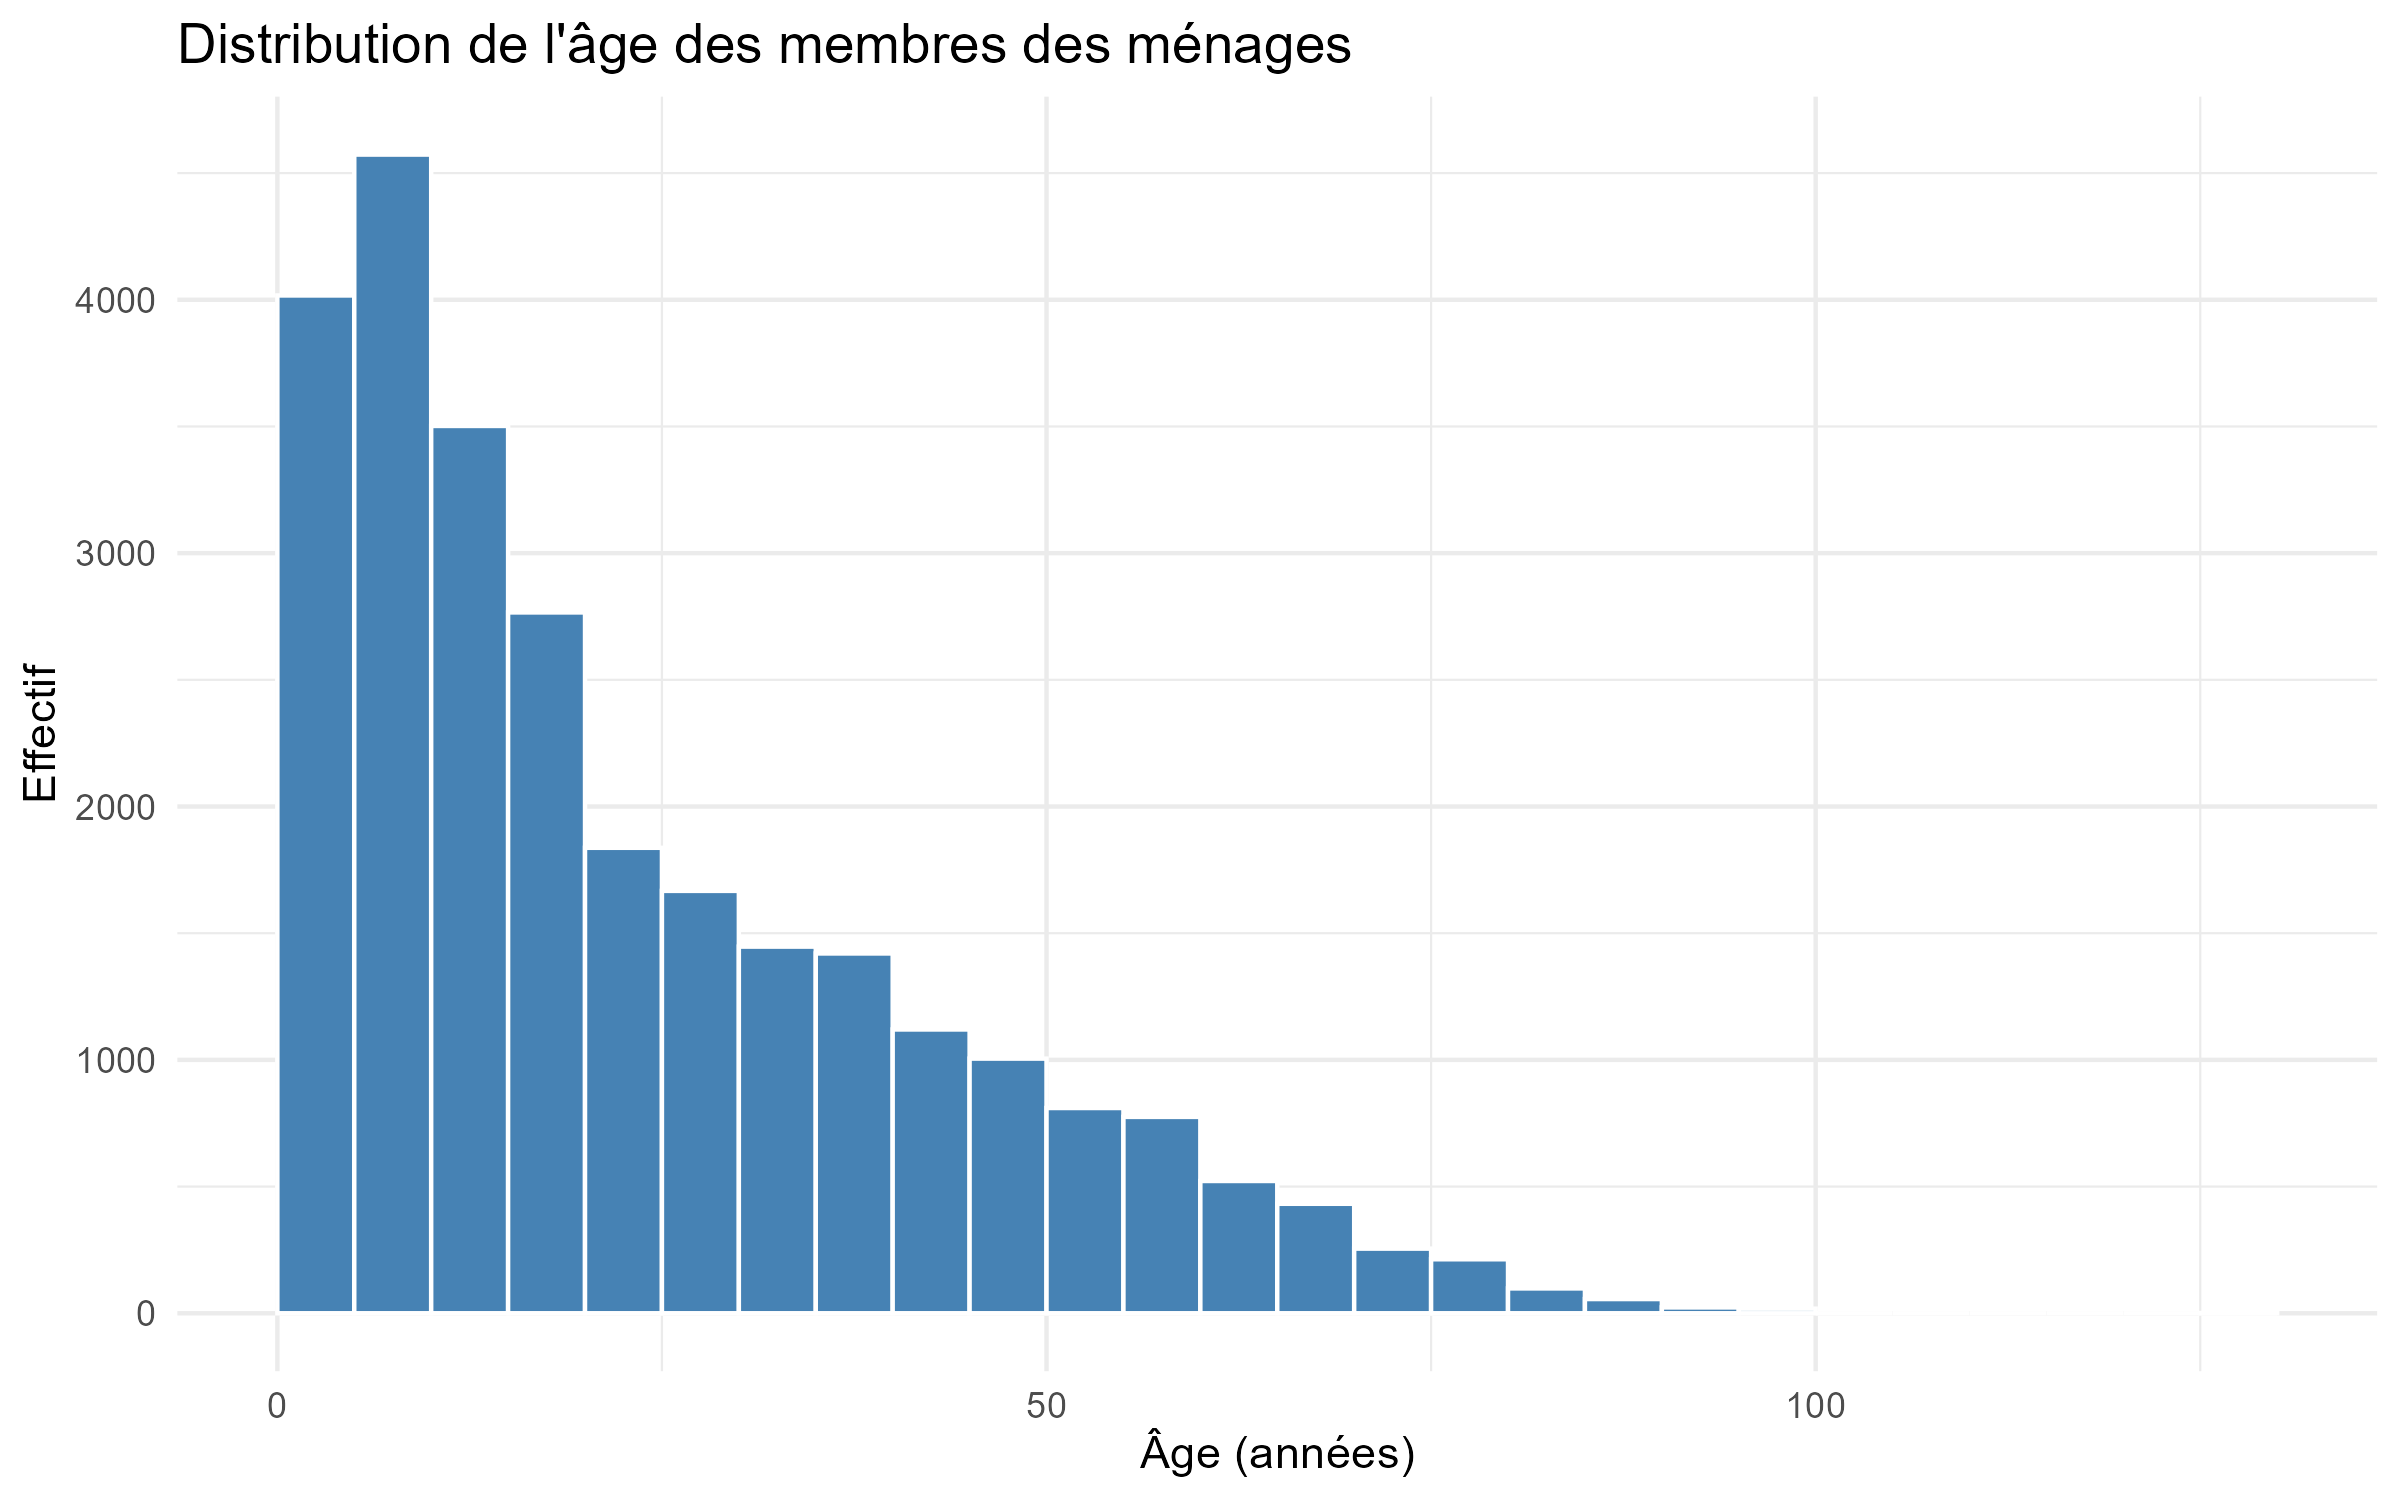
\includegraphics[width=1\linewidth]{../outputs/graphs/histogramme_age} \end{center}

\begin{center}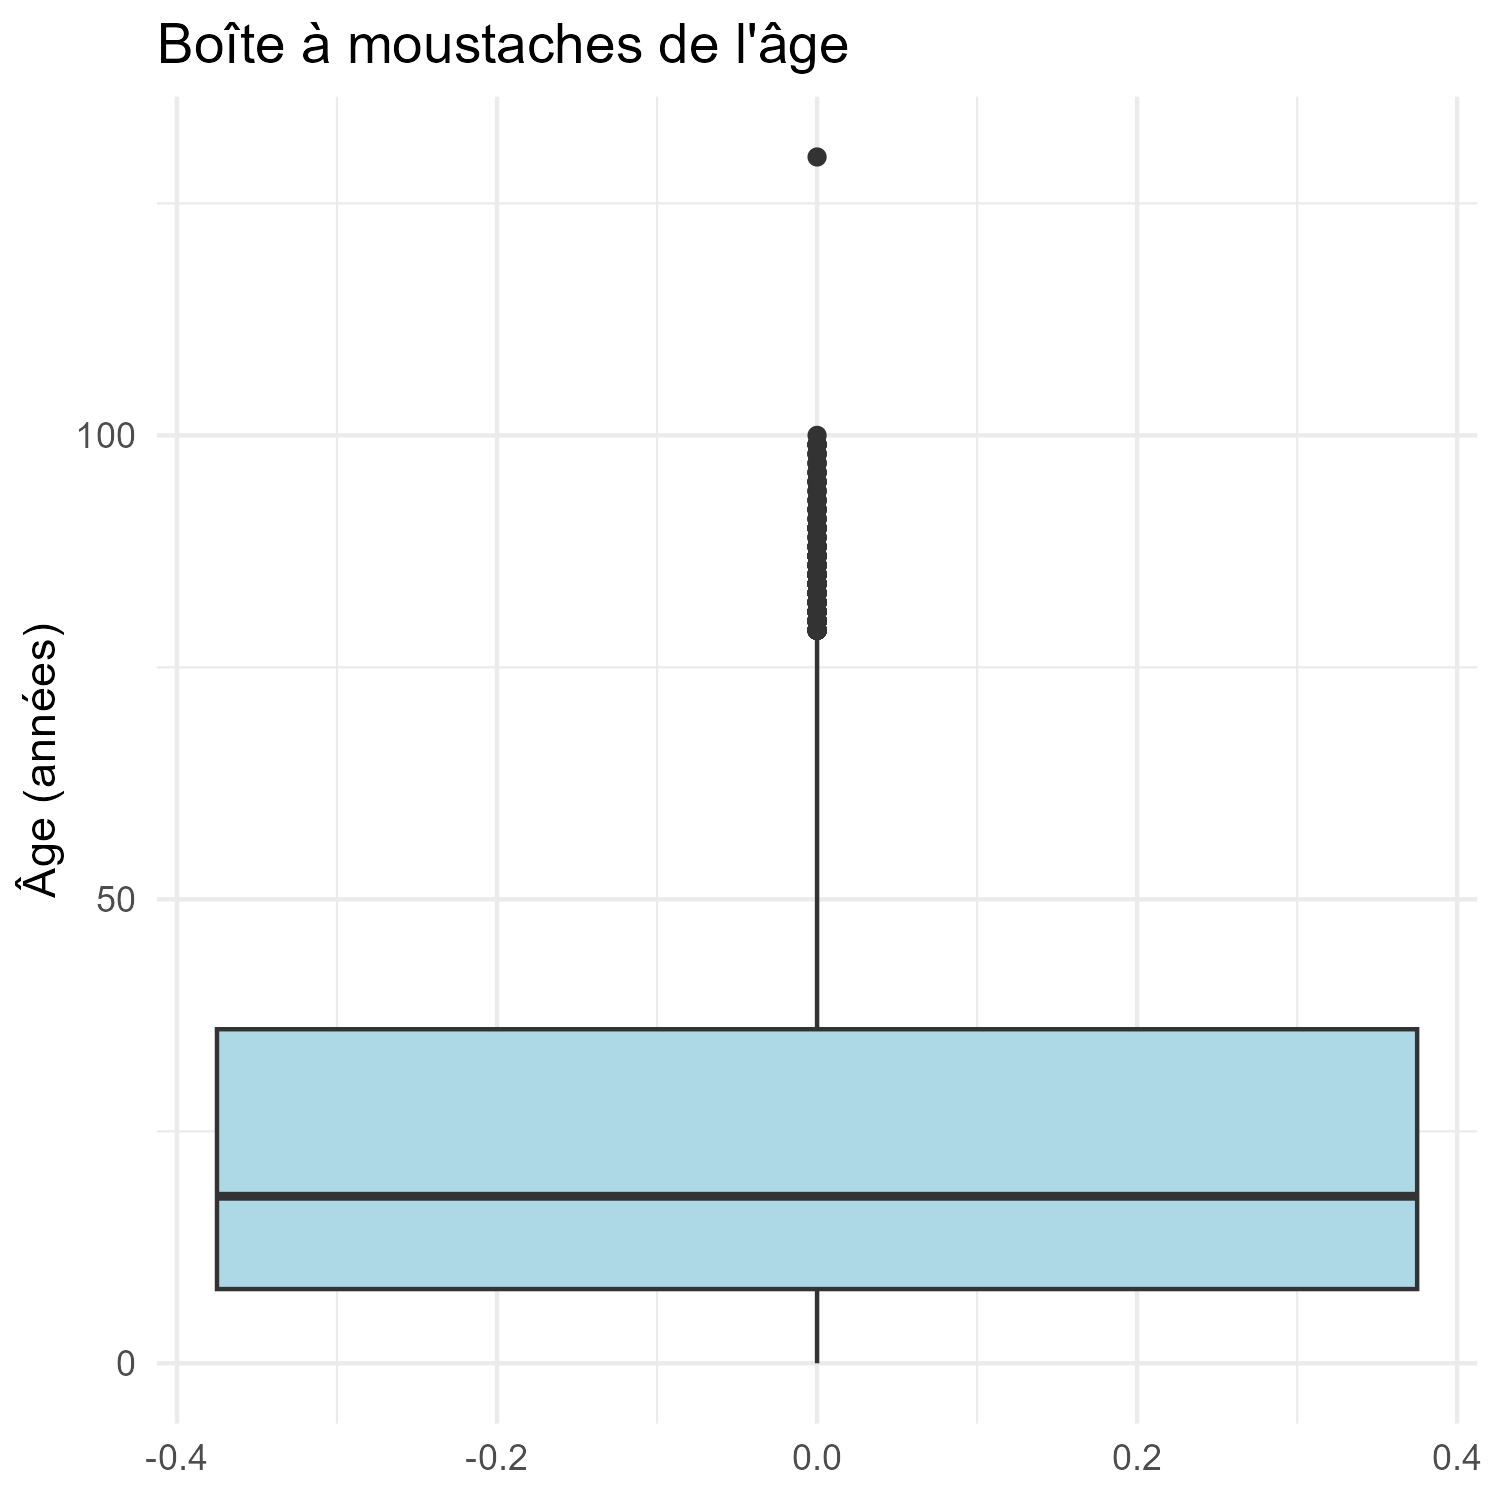
\includegraphics[width=1\linewidth]{../outputs/graphs/boxplot_age} \end{center}

L'histogramme montre une forte concentration des effectifs dans les
premières classes d'âge avec un pic chez les 0--4 ans, puis une
décroissance progressive typique d'une population jeune. Le boxplot
confirme la présence de valeurs extrêmes aux âges élevés et la médiane
basse à 18 ans.

\subsection{Pyramide des Âges par
Sexe}\label{pyramide-des-uxe2ges-par-sexe}

La pyramide des âges (groupes quinquennaux) visualise la structure par
sexe de la population enquêtée.

\begin{center}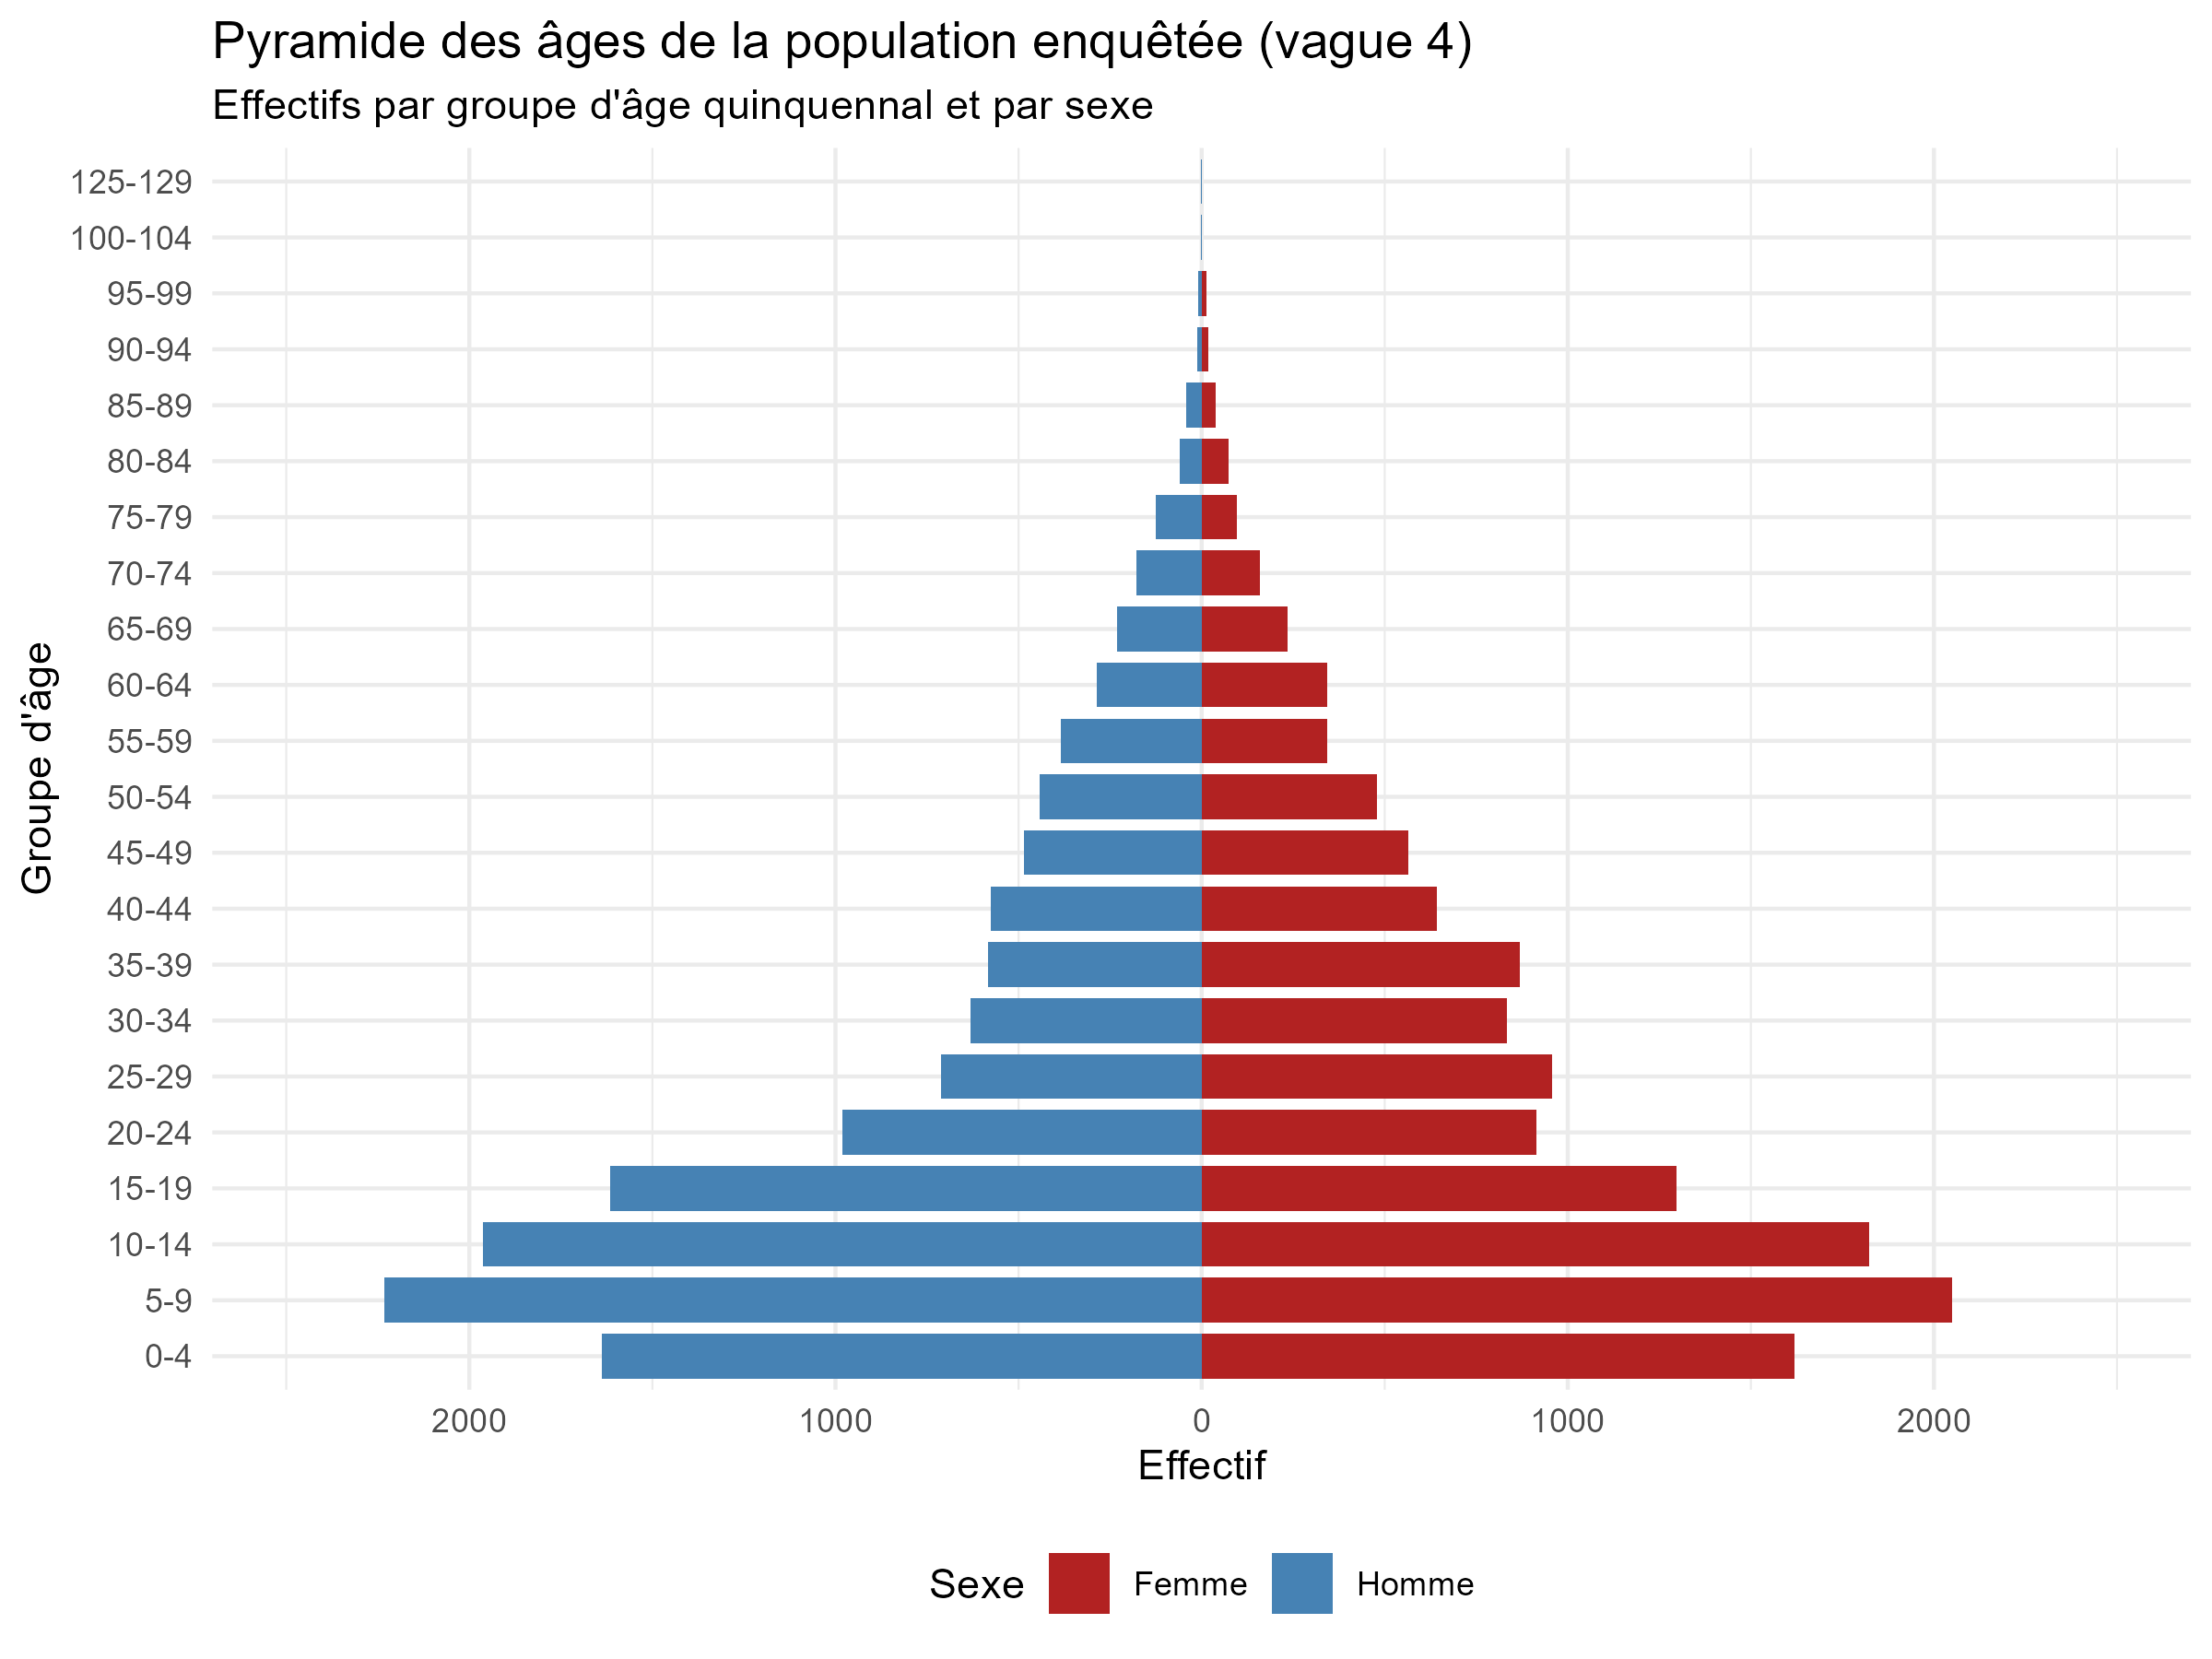
\includegraphics[width=1\linewidth]{../outputs/graphs/pyramide_ages} \end{center}

La pyramide présente une base large (classe 0--4 ans la plus fournie
dérrière 5--9 et 10--14), caractéristique d'une population jeune à forte
natalité. Ce profil suit une forme expansive typique des pays en
développement, où chaque génération est plus nombreuse que la
précédente. On observe un déséquilibre entre les sexes dans les classes
d'âge actives (15--30 ans), où les hommes sont plus nombreux,
probablement en raison d'une migration masculine temporaire vers les
zones d'emploi. À partir de 30 ans, les femmes deviennent
progressivement plus nombreuses, conformément aux tendances
démographiques liées à une espérance de vie féminine plus élevée.

\subsection{Lien de Parenté}\label{lien-de-parentuxe9}

La variable \texttt{s1q3} a été regroupée en quatre catégories : Chef,
Conjoint, Enfant, Autre.

\begin{longtable}[]{@{}lrlrr@{}}
\caption{Fréquences des liens de parenté avec IC à 95 \%}\tabularnewline
\toprule\noalign{}
relation & n & prop\_label & ic\_low & ic\_high \\
\midrule\noalign{}
\endfirsthead
\toprule\noalign{}
relation & n & prop\_label & ic\_low & ic\_high \\
\midrule\noalign{}
\endhead
\bottomrule\noalign{}
\endlastfoot
Enfant & 14636 & 55.1\% & 0.545 & 0.557 \\
Chef & 4980 & 18.8\% & 0.183 & 0.192 \\
Conjoint & 4273 & 16.1\% & 0.156 & 0.165 \\
Autre & 2668 & 10\% & 0.097 & 0.104 \\
\end{longtable}

\begin{center}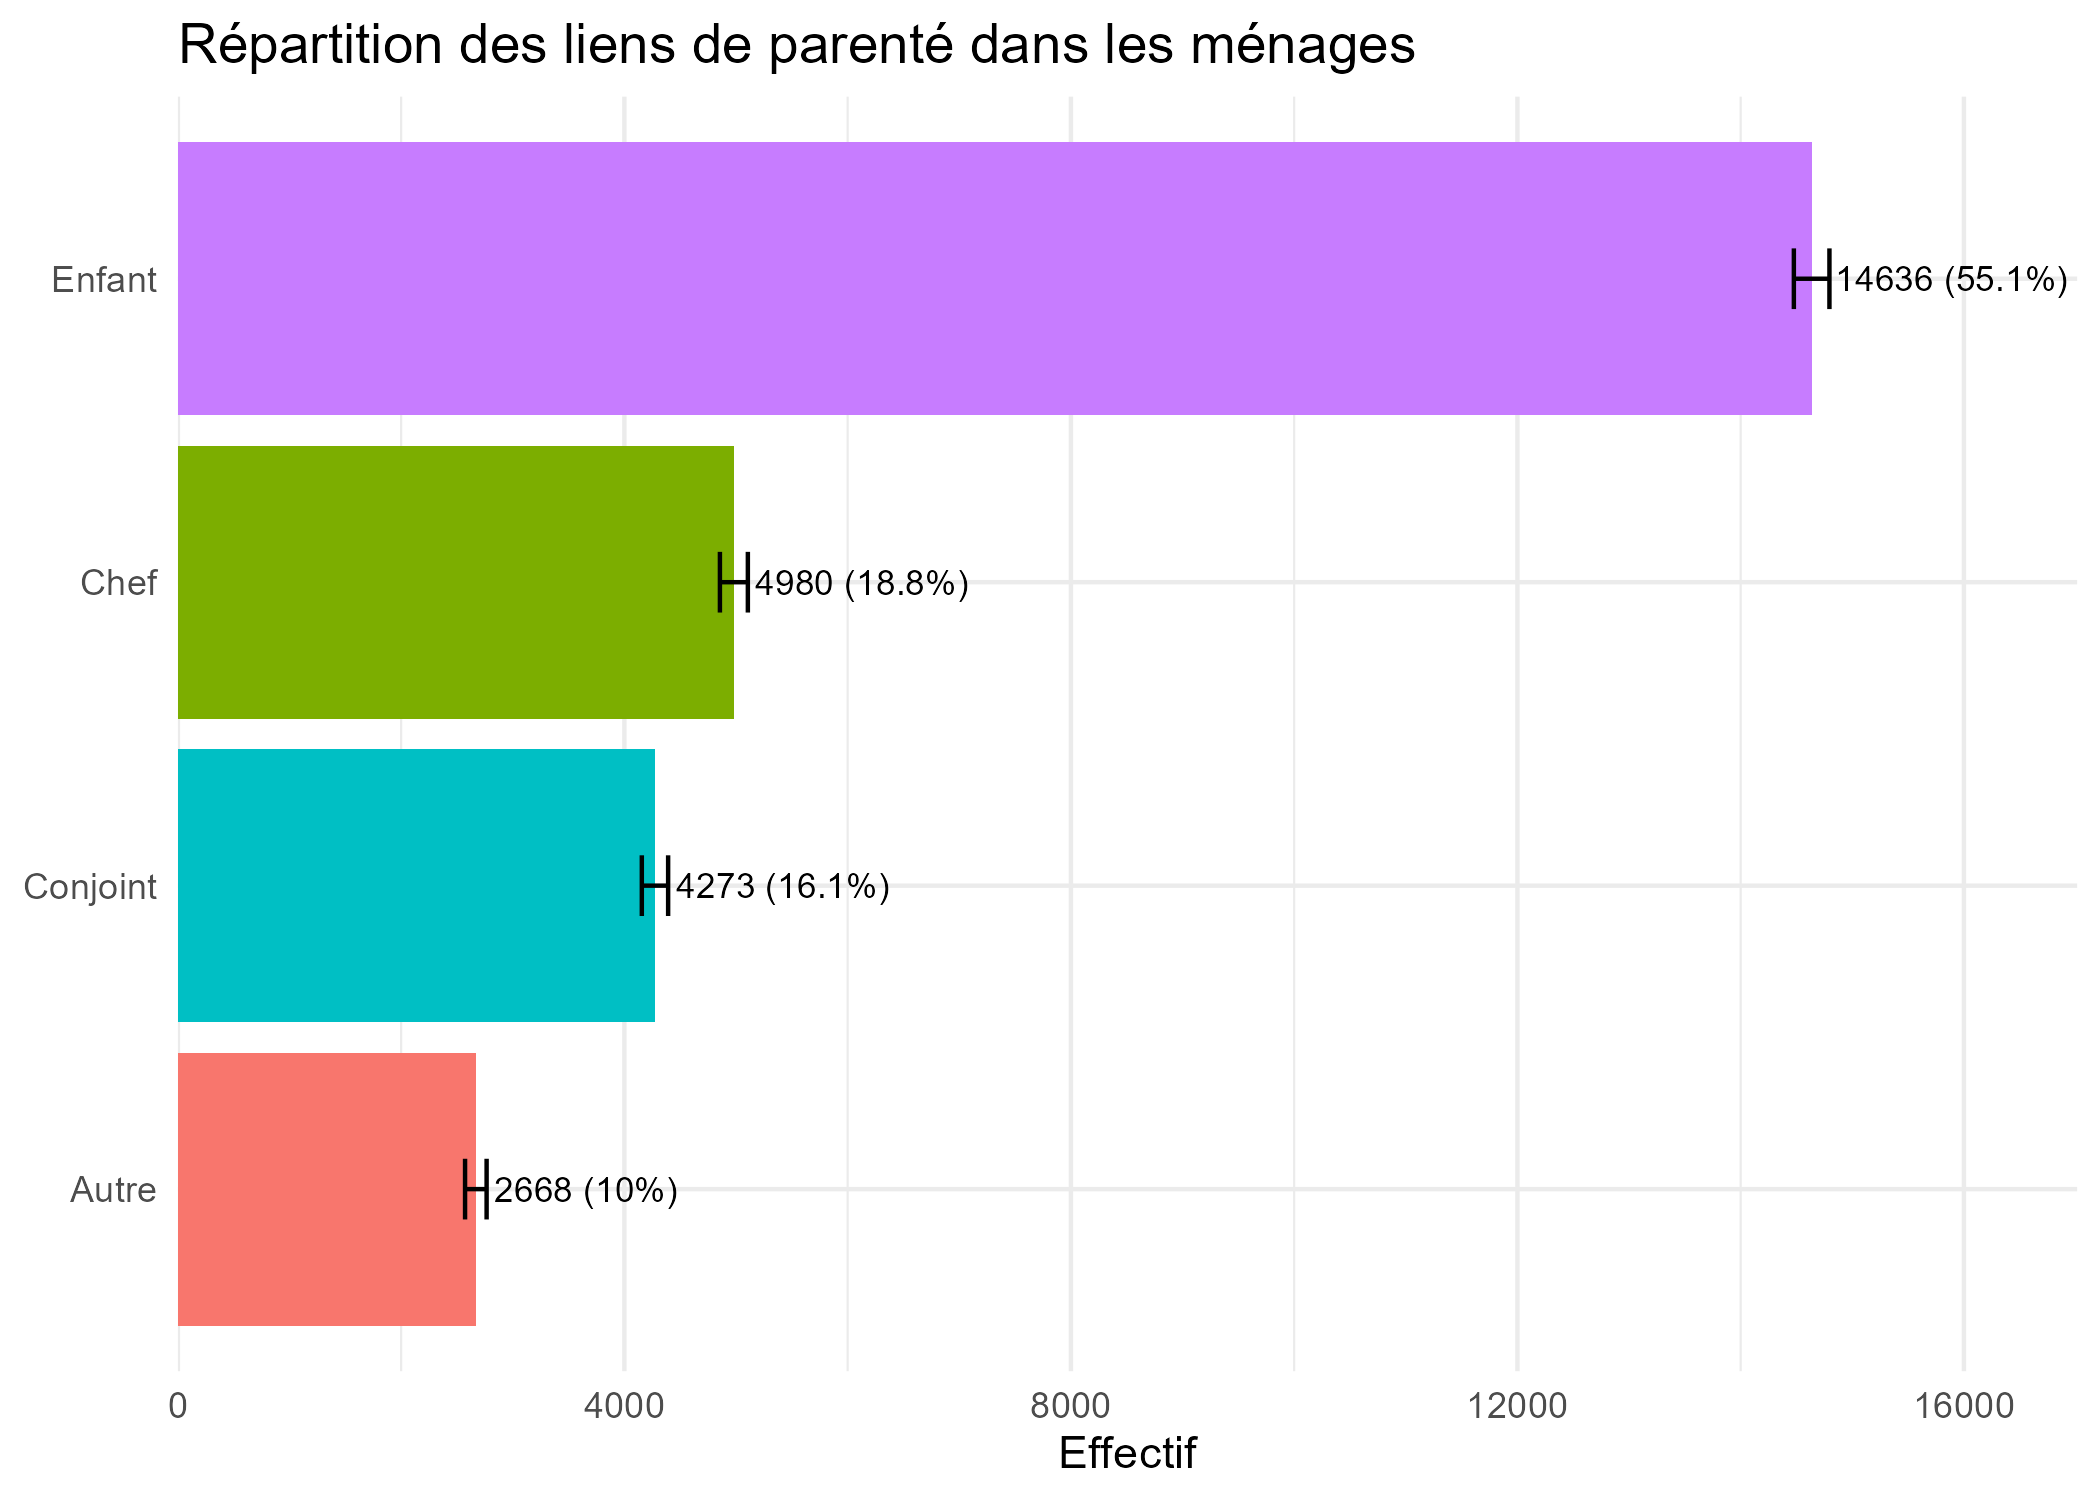
\includegraphics[width=1\linewidth]{../outputs/graphs/lien_parente_barplot} \end{center}

Les enfants représentent 55,1 \% des membres enquêtés, soit plus de la
moitié de la population, ce qui confirme la jeunesse de la structure
démographique nigériane. Les chefs de ménage constituent 18,8 \% de
l'échantillon et les conjoints 16,1 \%, proportions cohérentes avec une
structure familiale où chaque ménage compte en moyenne un chef, un
conjoint et plusieurs enfants. La catégorie Autre (10,0 \%) regroupe des
situations diverses telles que les parents, beaux-parents et
neveux/nièces, reflétant la fréquence des ménages élargis au Nigeria.

\subsection{Taille des Ménages et Comparaison Rural /
Urbain}\label{taille-des-muxe9nages-et-comparaison-rural-urbain}

La taille des ménages a été calculée par décompte des individus membres
effectifs par \texttt{hhid}, conformément à la définition du ménage dans
l'enquête. Le recours à une échelle d'équivalence adulte n'est pas
approprié ici, cette dernière étant réservée aux analyses de
consommation ou de bien-être.

\begin{longtable}[]{@{}lrrrrrrrr@{}}
\caption{Taille des ménages selon le milieu de résidence}\tabularnewline
\toprule\noalign{}
zone & n\_menages & moyenne & mediane & ecart\_type & Q1 & Q3 & min &
max \\
\midrule\noalign{}
\endfirsthead
\toprule\noalign{}
zone & n\_menages & moyenne & mediane & ecart\_type & Q1 & Q3 & min &
max \\
\midrule\noalign{}
\endhead
\bottomrule\noalign{}
\endlastfoot
Rural & 3385 & 6.4 & 6 & 3.8 & 4 & 8 & 1 & 33 \\
Urbain & 1595 & 5.5 & 5 & 3.3 & 3 & 7 & 1 & 27 \\
\end{longtable}

En zone rurale (3 385 ménages), la taille moyenne est de 6,4 personnes
(médiane 6), avec un écart-type de 3,8 et un maximum de 33 personnes. En
zone urbaine (1 595 ménages), elle est plus faible : 5,5 personnes en
moyenne (médiane 5), écart-type 3,3, maximum 27. Le test de
Wilcoxon-Mann-Whitney confirme une différence très significative entre
les deux distributions (p \textless{} 2,2e-16). La taille d'effet (r =
0,12) est qualifiée de faible selon les conventions de Cohen, indiquant
que si la différence est statistiquement robuste, son amplitude pratique
reste modeste et que d'autres facteurs tels que le niveau d'éducation,
l'accès aux services, la fécondité contribuent également à expliquer la
composition des ménages.

\begin{center}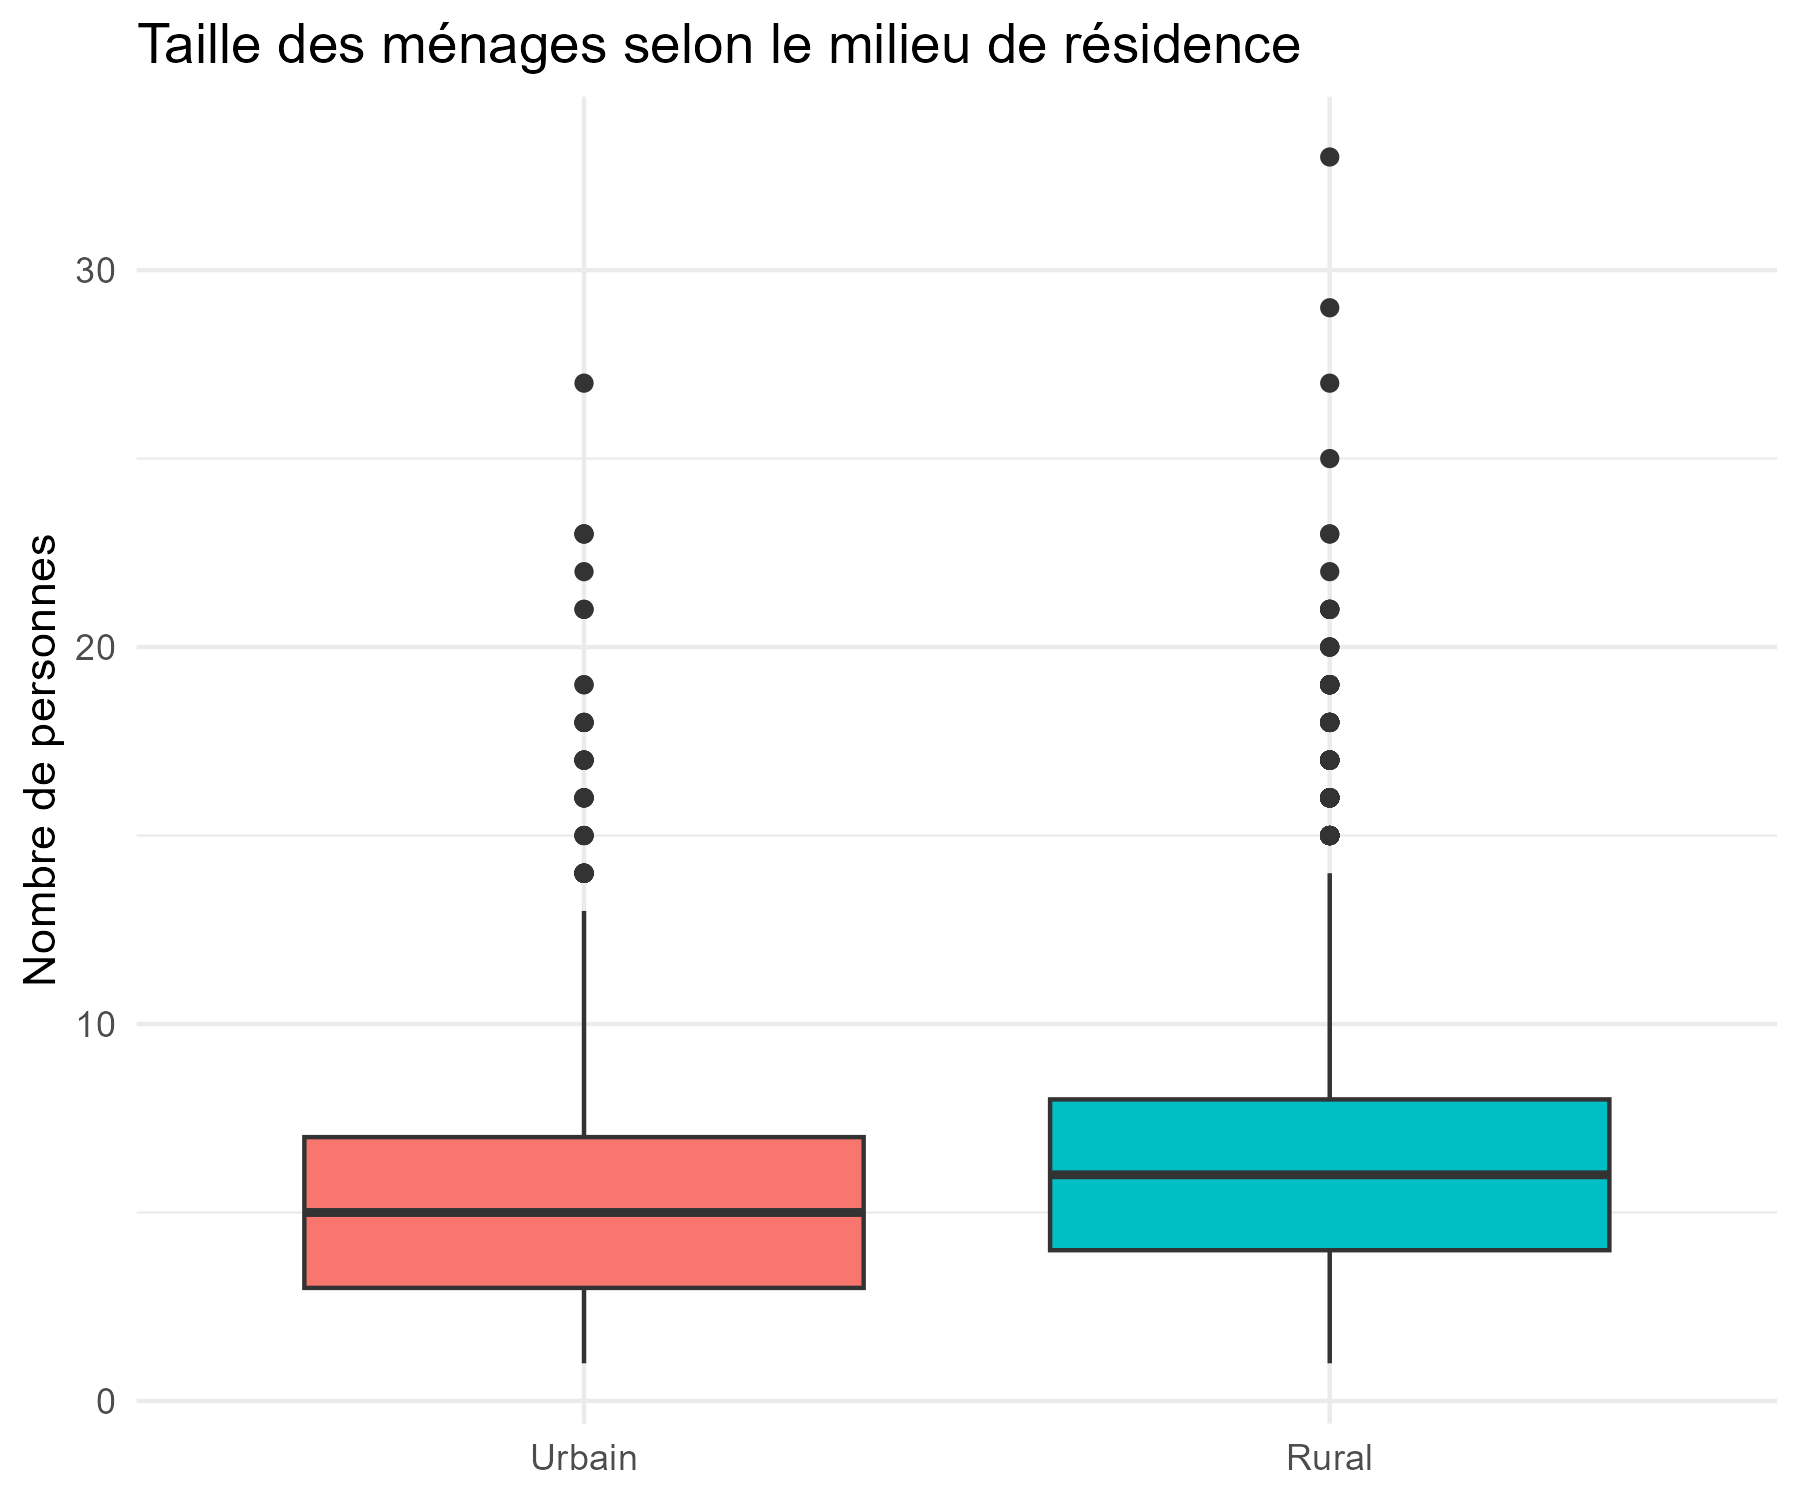
\includegraphics[width=1\linewidth]{../outputs/graphs/boxplot_taille_menage_par_zone} \end{center}

\begin{center}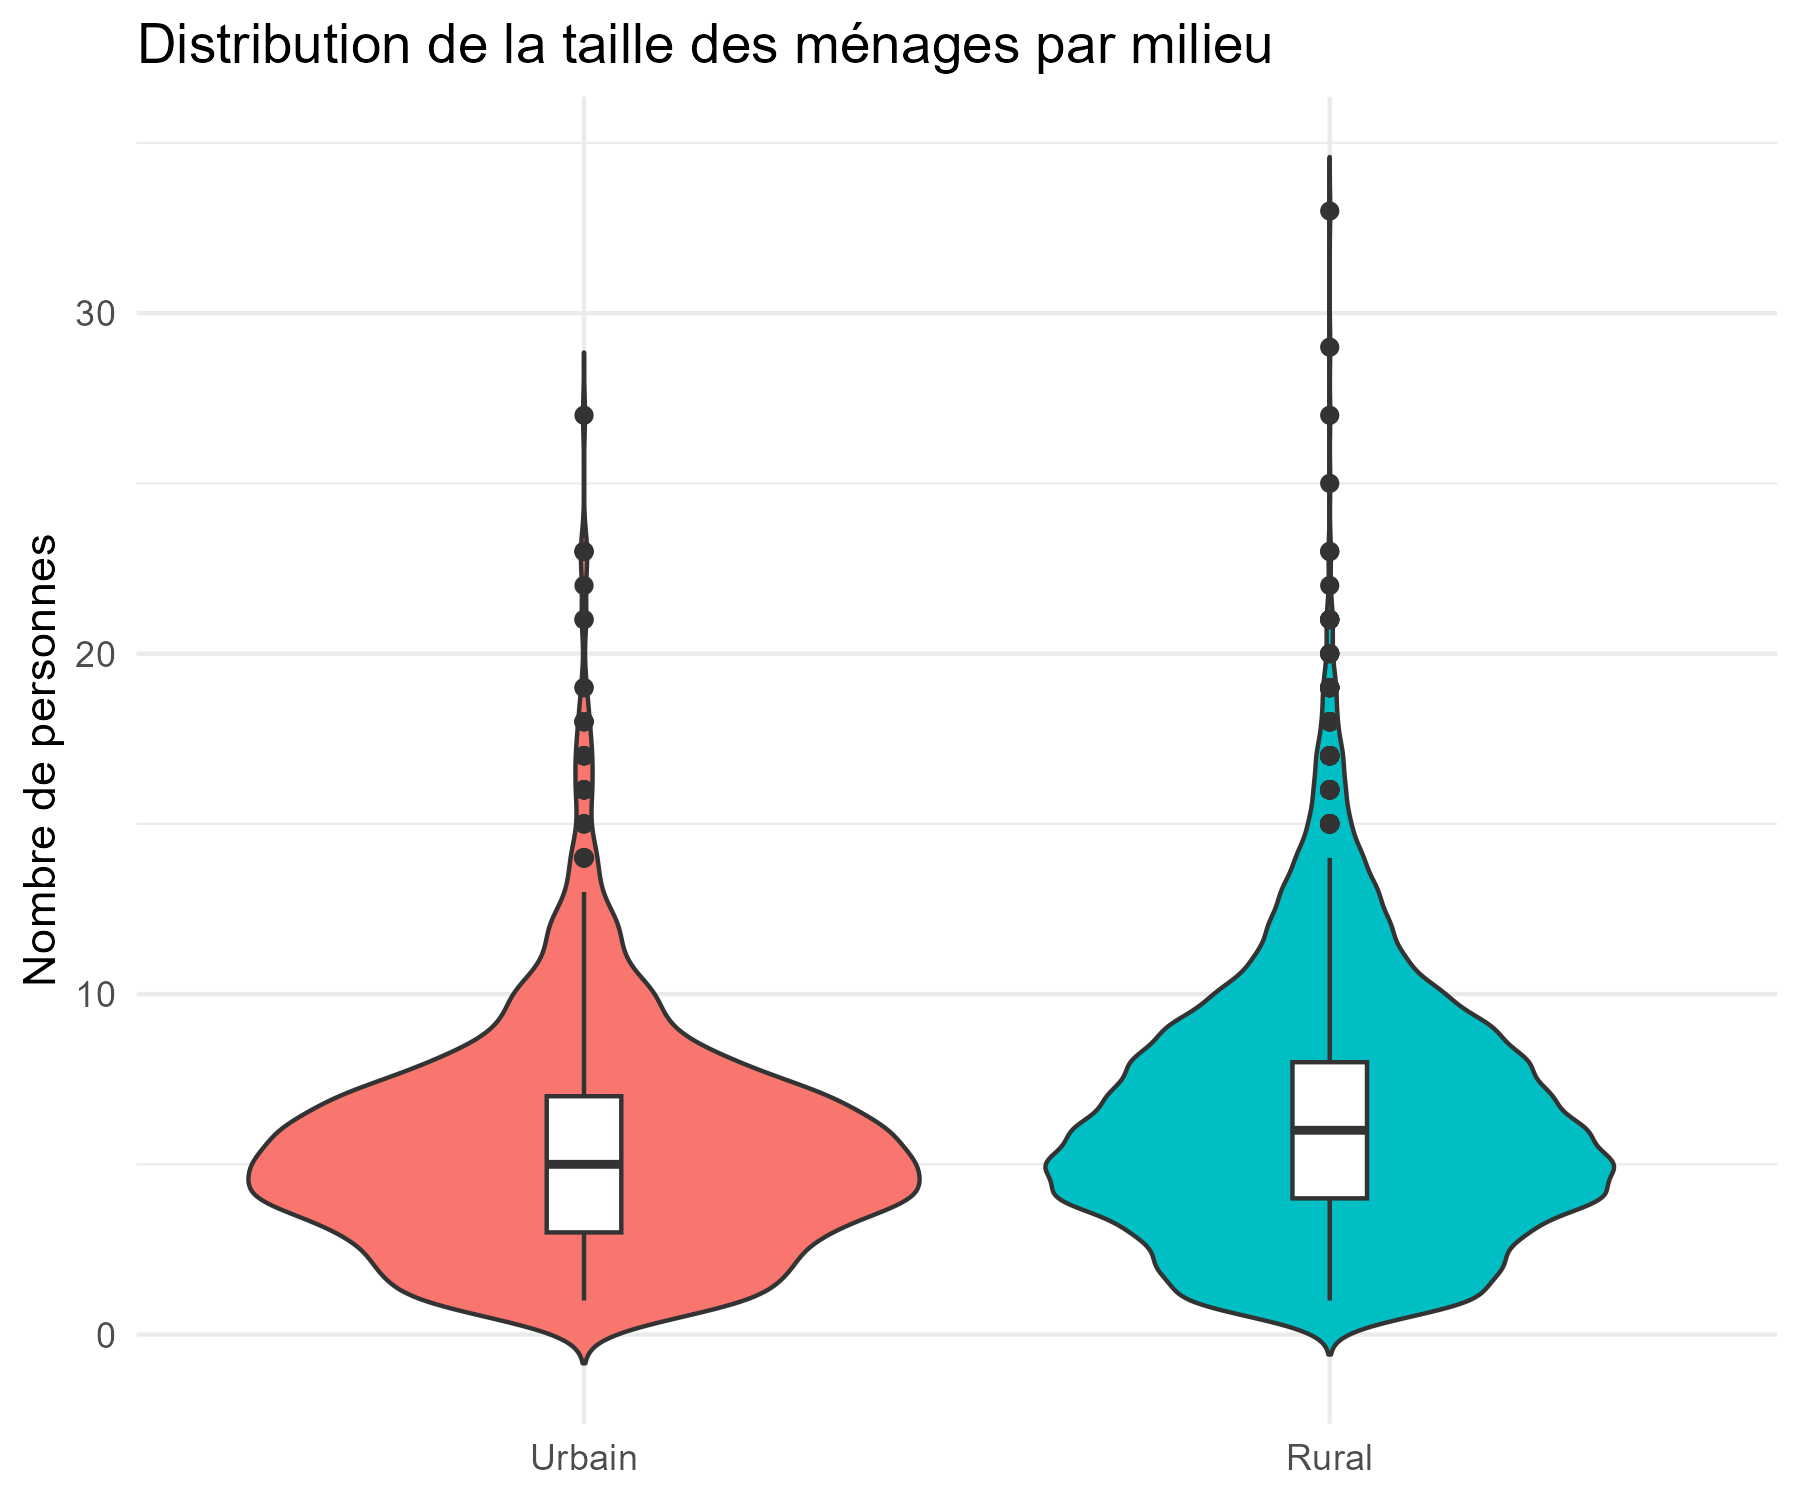
\includegraphics[width=1\linewidth]{../outputs/graphs/violin_taille_menage_par_zone} \end{center}

Le boxplot montre des médianes distinctes (6 vs 5) et une dispersion
plus forte en milieu rural. Le violin plot confirme une asymétrie à
droite plus marquée en zone rurale, avec une queue de distribution plus
étendue traduisant la présence de ménages très nombreux.

\subsection{Tableau Récapitulatif
Stratifié}\label{tableau-ruxe9capitulatif-stratifiuxe9}

Le tableau ci-dessous synthétise les principales caractéristiques
démographiques selon la zone de résidence.

\begingroup\fontsize{10}{12}\selectfont

\begin{longtable}[t]{lcccc}
\caption{\label{tab:tab_recap}Caractéristiques démographiques des ménages selon la zone}\\
\toprule
Caractéristique & Overall
N = 26 557 & | Urbain
N = 7 56 & | Rural
N = 18 9 & 0 | p-val\\
\midrule
\cellcolor{gray!10}{Sexe} & \cellcolor{gray!10}{} & \cellcolor{gray!10}{} & \cellcolor{gray!10}{} & \cellcolor{gray!10}{}\\
\hspace{1em}Homme & 13 189 (50\%) & 3 730 (49\%) & 9 459 (50\%) & \\
\hspace{1em}\cellcolor{gray!10}{Femme} & \cellcolor{gray!10}{13 368 (50\%)} & \cellcolor{gray!10}{3 837 (51\%)} & \cellcolor{gray!10}{9 531 (50\%)} & \cellcolor{gray!10}{}\\
Âge (années) & 24,0 (19,7) & 25,0 (19,4) & 23,6 (19,8) & \\
\cellcolor{gray!10}{Taille du ménage} & \cellcolor{gray!10}{7 (5, 10)} & \cellcolor{gray!10}{6 (5, 9)} & \cellcolor{gray!10}{8 (5, 11)} & \cellcolor{gray!10}{}\\
\bottomrule
\end{longtable}
\endgroup{}

L'âge moyen est légèrement plus élevé en ville (25,5 ans contre 23,2 ans
en milieu rural), différence significative au test de Wilcoxon,
probablement liée à une migration des jeunes adultes vers les zones
urbaines. La répartition hommes/femmes est comparable dans les deux
zones (environ 47--48 \% d'hommes), sans différence significative
(chi-deux, p = 0,4), ce qui indique une structure de genre homogène
entre milieux. La taille des ménages reste la caractéristique la plus
discriminante entre les deux zones, comme analysé à la section
précédente.

\section{Discussion}\label{discussion}

Les analyses confirment une structure démographique typique d'un pays en
développement à forte croissance démographique. La population est très
jeune (âge médian 18 ans) avec une forte proportion d'enfants (55,1 \%
des membres enquêtés), ce qui se traduit par une pyramide des âges à
base large caractéristique d'une fécondité élevée. Les ménages ruraux
sont significativement plus grands que les ménages urbains (6,4 contre
5,5 personnes en moyenne), reflet de structures familiales élargies,
d'une fécondité plus forte et d'un moindre accès aux services de
planification familiale en zone rurale. La déséquilibre observé dans les
classes d'âge actives (15--30 ans), où les hommes sont surreprésentés,
suggère l'existence de flux migratoires masculins temporaires, phénomène
courant dans les économies en développement.

Au-delà des disparités quantitatives, ces résultats soulèvent la
question de la pression démographique sur les ressources des ménages.
Une population majoritairement composée d'enfants et de jeunes
dépendants implique un ratio de dépendance élevé, susceptible de peser
sur les capacités d'épargne et d'investissement des ménages, en
particulier en milieu rural où les ménages sont déjà plus nombreux.

\textbf{Limites :}

\begin{itemize}
\item
  L'analyse repose sur une coupe transversale (vague 4) ; elle ne permet
  pas d'étudier les évolutions temporelles de la structure
  démographique.
\item
  La catégorie « Autre » pour le lien de parenté regroupe des situations
  diverses ; une ventilation plus fine pourrait apporter des nuances sur
  la prévalence des ménages élargis.
\item
  La valeur maximale d'âge déclarée (130 ans) n'a pas été corrigée dans
  cette analyse ; une procédure de nettoyage des valeurs aberrantes
  d'âge pourrait améliorer la qualité des statistiques descriptives.
\end{itemize}

\section{Conclusion}\label{conclusion}

Ce travail a permis de dresser un portrait démographique détaillé des
ménages nigérians à partir de la vague 4 du GHS Panel. Il met en
évidence une population très jeune, des ménages ruraux significativement
plus grands, et une structure familiale dominée par les enfants. Le
déséquilibre de genre observé dans les classes d'âge actives suggère des
flux migratoires masculins temporaires. Ces résultats constituent une
base solide pour des analyses ultérieures portant sur l'éducation, la
santé ou l'agriculture, qui exploiteront d'autres modules de l'enquête.

\end{document}
